\chapter{Results}\label{chap:results}

This chapter will present the outcomes of the design and development phase.
First, the artifact is presented from a user's point of view, showcasing functionality with screenshots.
Then, the artifact's design will be presented from an architectural view, and the protocol will be presented last.\\

The results will also present the measures taken for making the \gls{open source} project viable, and something a developer community may want to develop and maintain further.\\

Evaluation of the results is presented later, in \cref{chap:evaluation}.

\section{Software Artifact: Tree Editor Extension for Ecore in Gitpod}

This is of interest for a stakeholder, and someone aiming to do further research on this design.

The output of the development phase is an artifact which is a \gls{VSCode} extension.
The artifact is a \texttt{.vsix} file, and can be installed in a \gls{Gitpod} workspace.
The following results are from \gls{Gitpod} using \gls{VSCode} as the editor frontend, not \gls{Theia}\footnote{VSCode is supposed to become the default for Gitpod in the future, instead of Theia~\cite{georgetsiolisMenuEntryGitpod2019}.}.
One way to install it\footnote{The ``best'' way is to publish the extension to OpenVSX, and search for it in the extensions panel.}, is to upload the \texttt{.vsix} file to the workspace, right clicking on it and selecting ``Install Extension VSIX''.
When installed in the \acrshort{IDE}, it is shown in the extensions panel as \textit{Ecore Tree-editor}, shown in \cref{fig:gitpod-ext-installed}.

\begin{figure}[H]  % order of priority: h here, t top, b bottom, p page
  \centering
  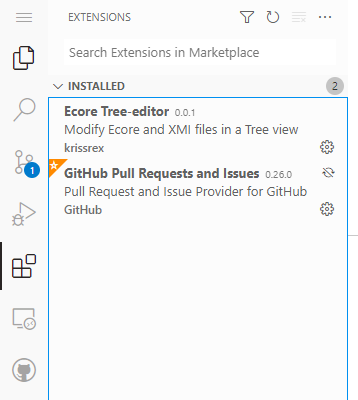
\includegraphics[width=0.6\textwidth]{figures/gitpod-vscode-extensions-installed.png}
  \caption[Tree Editor Extension installed in Gitpod]{The extension is installed as \textit{Ecore Tree-editor} in Gitpod with VSCode.}\label{fig:gitpod-ext-installed}
\end{figure}

\subsection{Custom Editor}

This extension adds a new Custom Editor, which is automatically opened when the user opens a \texttt{.ecore}, \texttt{.genmodel} or \texttt{.xmi} file.
The model file is loaded and transformed by the extension, and presented as a tree to the user.

\begin{figure}[H]  % order of priority: h here, t top, b bottom, p page
  \centering
  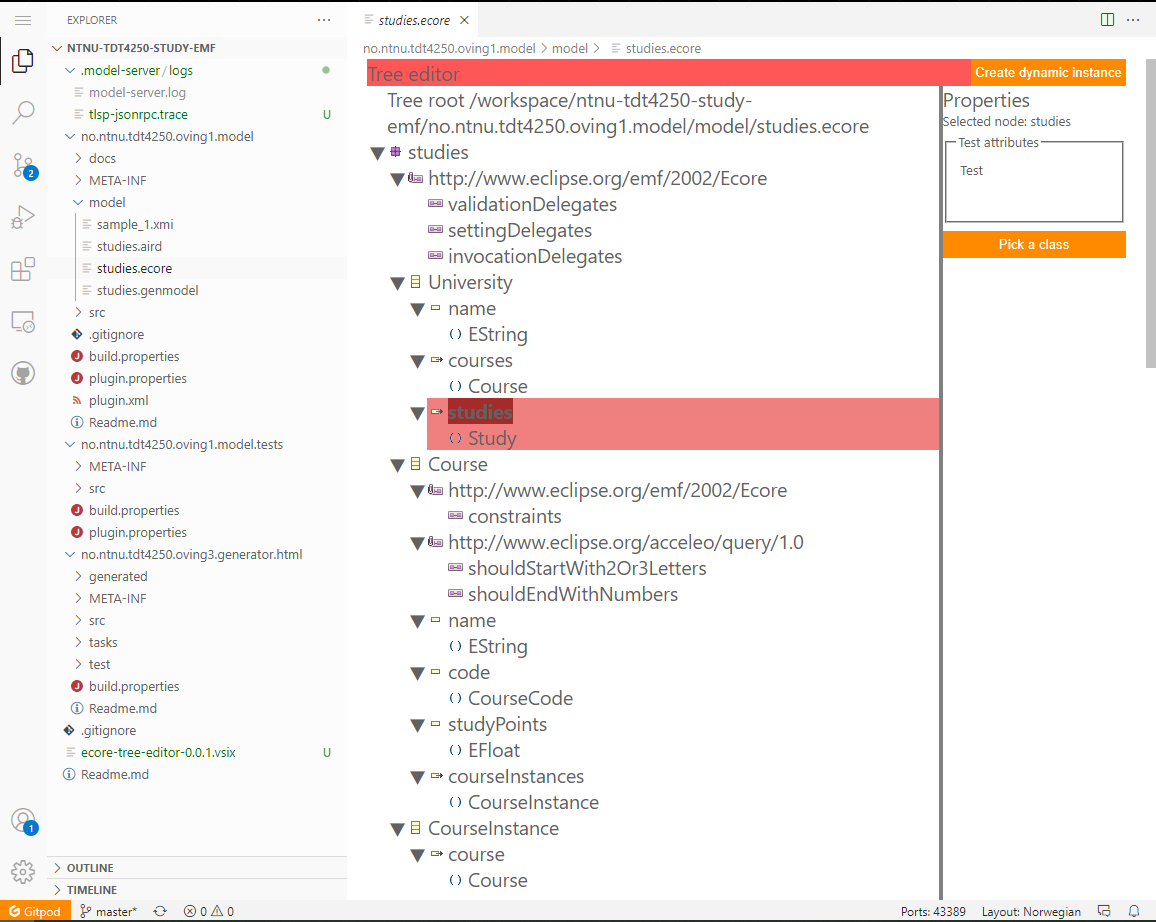
\includegraphics[width=\textwidth]{figures/gitpod-vscode-ecore-editor-studyemf.png}
  \caption[Tree Editor Extension showing studies.ecore]{The Tree Editor Extension has opened a Custom Editor for the \texttt{studies.ecore} file.}\label{fig:gitpod-ext-tree-ecore}
\end{figure}

\paragraph{Example model}
An \gls{Ecore} model made in \gls{TDT4250} in 2019 has been used as an example to demonstrate the artifact.
The \texttt{.ecore} file is opened in \cref{fig:gitpod-ext-tree-ecore}.
This figure shows three columns, from left to right: the default \gls{VSCode} file explorer, the custom editor's master layout (tree structure), and the custom editor's detail layout (properties sheet).

\paragraph{Action bar}
There is also a red action bar at the top, with an orange action button to create a new dynamic instance.
The action buttons shown will vary, depending on what the selected node is.
The orange color of the button is coming from the color theme of the \gls{VSCode} editor.
With a dark theme, this action button could be blue, for example.

\paragraph{Master layout}
The master layout can show multiple roots.
In this document,  single root is shown for the ``studies.ecore'' file.
The root node is a ``studies'' package, with children displayed below.
This node has a label, ``studies'', and a specific icon indicating it is a package --- the purple box with a cross.
The icons used are the same ones used in \gls{Eclipse} for the Sample Reflective Ecore Editor (see \cref{sec:sample-reflective-editor}), and depend on the type of node.

Clicking the black triangle next to a node will collapse it, hiding its children and rotating the triangle 90 degrees counter-clockwise.

Inside the master layout, a node is selected in dark red, with the label ``studies''.
Its child node ``Study'' is also highlighted, in a lighter red.
(Note that the colors of selected nodes were arbitrarily chosen during development, and could be changed to give more contrast with the node's label.)
A node can be selected by clicking on it, and holding \texttt{ctrl} will add to the selection, allowing multiple nodes to be selected.

Dragging a node in the hierarchy and dropping it on a node, should change this node's parent.
Right clicking a node will open a context menu, with the possible children nodes to add.
Dropping a node on an invalid parent will be prevented, by using a hierarchy schema, and indicated by changing the mouse cursor to a ``forbidden'' icon\footnote{Note that drag-and-drop and node creation are not currently implemented, only accounted for by the design, by using a hierarchy schema.}.


\paragraph{Detail layout}
The detail layout has a property sheet, currently showing a unfinished example form.
This layout should use the \textit{JSON-Forms} library to render properties, based on the node's properties and a \textit{UI schema} for that node type.


\subsection{IDE Commands}

The extension also provides Commands to \gls{VSCode}.
These are actions that can be invoked at any time.
The student can invoke them from the Command Palette\footnote{Press \texttt{F1}, or \texttt{ctrl + shift + P} (command on mac), or \texttt{Menu $\rightarrow$ View $\rightarrow$ Command palette}} by typing ``Ecore'' or another part of the command's name.
A screenshot is shown in \cref{fig:gitpod-ext-newmodel}, with a command to create a new model file.
This file will have the minimum \acrshort{XMI} contents required for a blank model.

\begin{figure}[H]  % order of priority: h here, t top, b bottom, p page
  \centering
  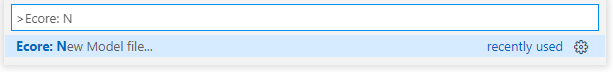
\includegraphics[width=\textwidth]{figures/gitpod-vscode-newmodel.png}
  \caption[Tree Editor Extension Custom Commands]{The Tree Editor Extension adds custom commands to the Command Palette. One of them is shown here, named \textit{Ecore: New Model file\ldots}.}\label{fig:gitpod-ext-newmodel}
\end{figure}

\subsection{Genmodel and Model Instance}

The editor can open a \texttt{.genmodel} file or a \texttt{.xmi} model instance file as well.
The GenModel is shown in \cref{fig:gitpod-ext-genmodel}, and the dynamic instance in \cref{fig:gitpod-ext-dynamic}.
This will show two roots in the editor, as the original \texttt{.ecore} model is related to the opened file.
One root is the GenModel or model instance, and the other root is the study model.

The GenModel editor is not specialized, so it renders the tree as any other \gls{Ecore} model.

\begin{figure}[H]  % order of priority: h here, t top, b bottom, p page
  \centering
  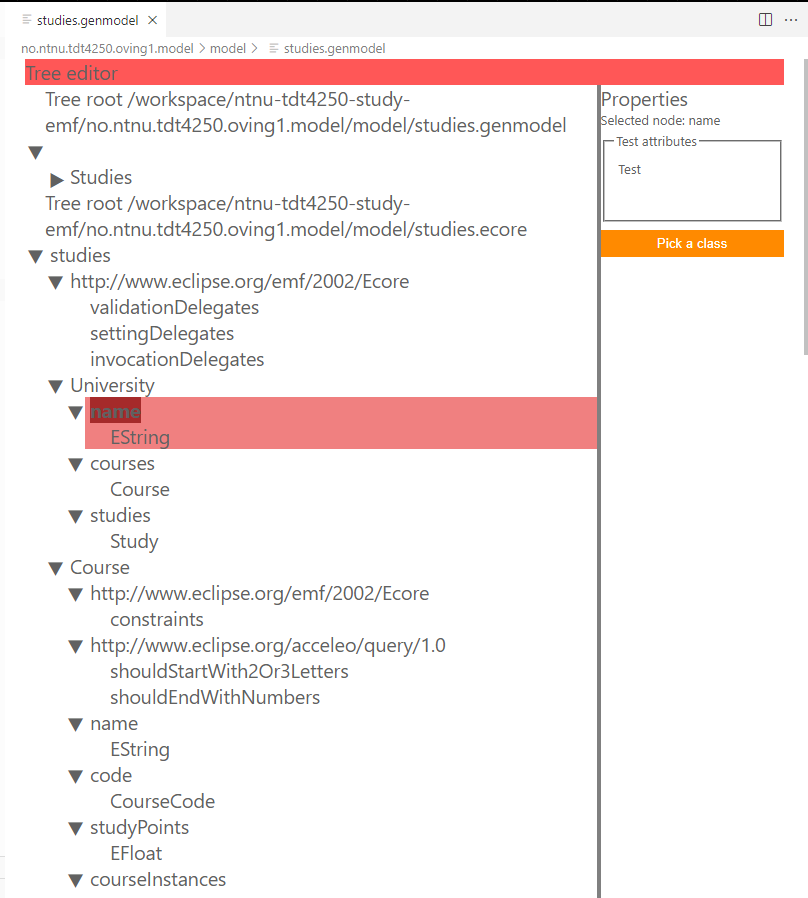
\includegraphics[width=\textwidth]{figures/gitpod-vscode-genmodel.png}
  \caption[Tree Editor Extension showing studies.genmodel]{The Tree Editor Extension with the \texttt{studies.genmodel} file open. It has two roots, the GenModel and the model. The GenModel is collapsed/hidden at the ``Studies'' node.}\label{fig:gitpod-ext-genmodel}
\end{figure}

\begin{figure}[H]  % order of priority: h here, t top, b bottom, p page
  \centering
  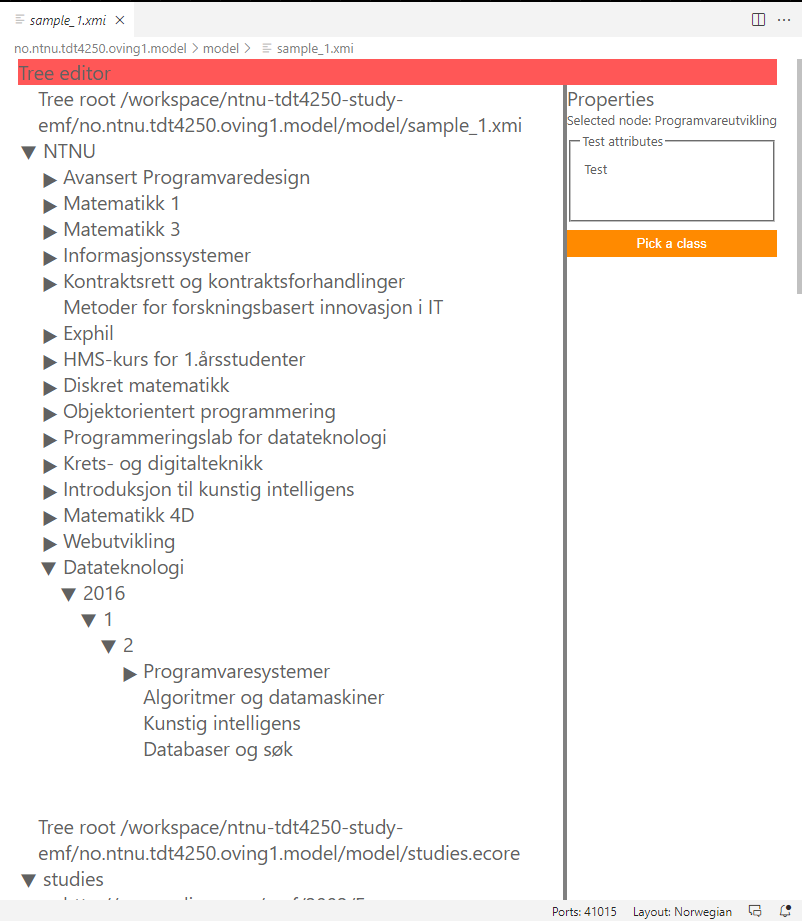
\includegraphics[width=\textwidth]{figures/gitpod-vscode-xmi-study-instance.png}
  \caption[Tree Editor Extension showing a dynamic instance]{The Tree Editor Extension with the \texttt{sample_1.xmi} dynamic instance open. This is data that conforms to the model defined in \texttt{studies.ecore}.}\label{fig:gitpod-ext-dynamic}
\end{figure}


\subsection{Configuration and Logging}

The extension has configuration options that a user can set.
One such option is the logging level, a threshold to hide log messages in the log panel.
The extension can also log internal events and messages to a Output panel in \gls{VSCode}, for the user to debug and identify errors.
The configuration and output panel are shown in \cref{fig:gitpod-ext-config-log}.

\begin{figure}[htbp]  % order of priority: h here, t top, b bottom, p page
  \centering
  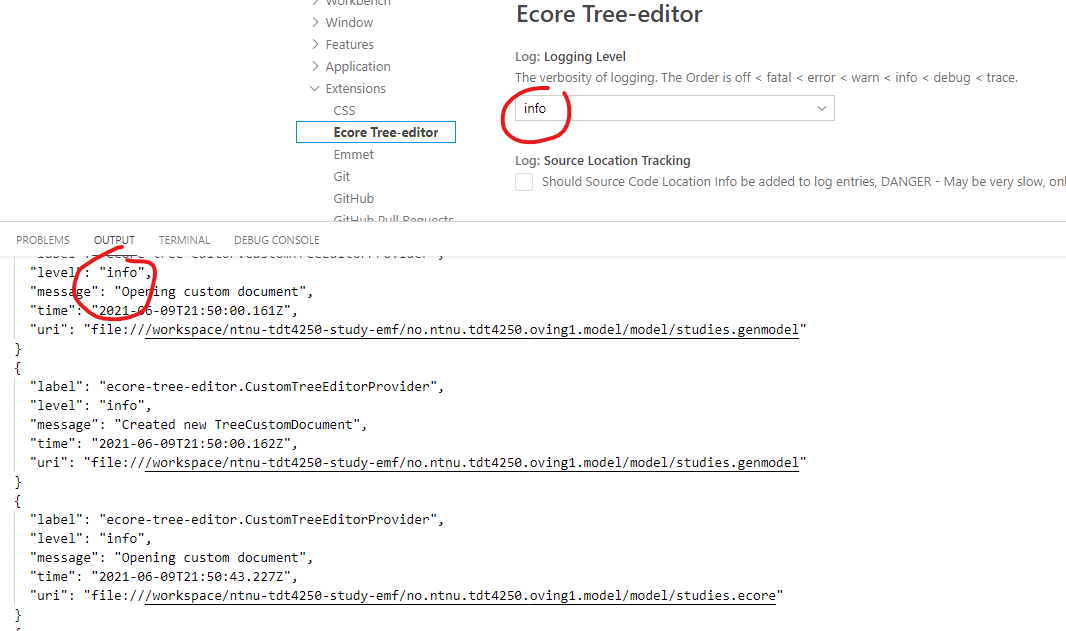
\includegraphics[width=\textwidth]{figures/gitpod-vscode-config-and-logging.png}
  \caption[Tree Editor Extension with configuration and logging]{The Tree Editor Extension adds configuration options to the \gls{VSCode} settings menu, shown in the top right.
  The extension also adds log outputs to a Output panel.
  The figure is annotated with two red circles.
  The upper circle is indicating the configuration option to filter the output based on log level.
  The lower circle is highlighting that same log level from a message in the output panel.}\label{fig:gitpod-ext-config-log}
\end{figure}


\iffalse{
% * Steps:
% 1. Sign up to Gitpod.io with GitHub user
% 2. Go to Settings. Set default IDE as VSCode. (It will be the default soon % % https://github.com/gitpod-io/gitpod/issues/3989#issuecomment-822246441)
% 3. Open %https://gitpod.io/#https://github.com/krissrex/ntnu-tdt4250-study-emf % to get a Workspace in gitpod with an EMF project. The Tree Language Server does % not support multi-workspace.
% 4. Build the extension locally to obtain a .vsix file (or download a build from % somewhere)
% 5. Upload the .vsix to the project workspace by drag-and-drop.
% 6. Right-click the .vsix file in VSCode/Gitpod, select "Install Extension VSIX".
% 7. Wait for "Completed installing Ecore Tree-editor extension from VSIX" popup % in bottom right corner.
% 8. Open folder with models: "no.ntnu.tdt4250.oving1.model/model"
% 9. Click model file: "studies.ecore"
% 10. Click genmodel file: "studies.genmodel"
% 11. Click dynamic instance file: "sample_1.xmi"
}
\fi

\FloatBarrier % Prevent figures running into the next section


\section{Design Artifact: Architecture for Tree Language Server Systems}

% TODO

* Architecturally significant requirements
* Architecture iterations
* Final architecture. C4 diagram (context, containers, components, code)

\begin{figure}[htbp]  % order of priority: h here, t top, b bottom, p page
  \centering
  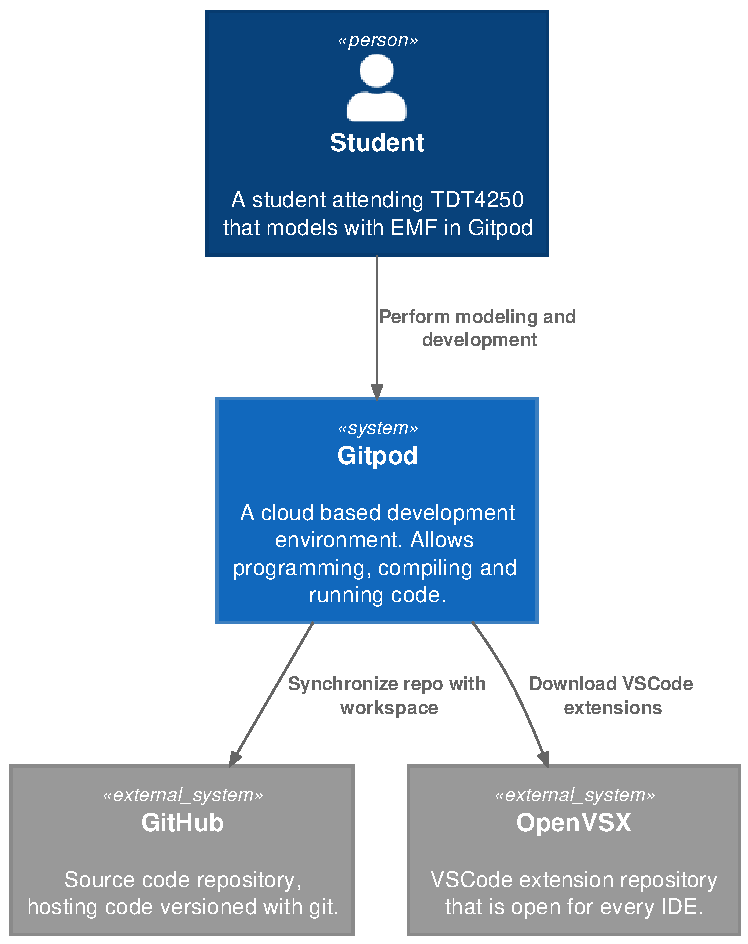
\includegraphics[width=\textwidth]{figures/plantuml/Gitpod_context.pdf}
  \caption[System context diagram for Gitpod]{A system context diagram for Gitpod. The extension will run inside the Gitpod service, used by a student to do modeling and developing. Gitpod uses git to synchronize code with GitHub. The extensions in Gitpod are downloaded from a service called OpenVSX.}\label{fig:gitpod-system-context}
\end{figure}

\begin{figure}[htbp]  % order of priority: h here, t top, b bottom, p page
  \centering
  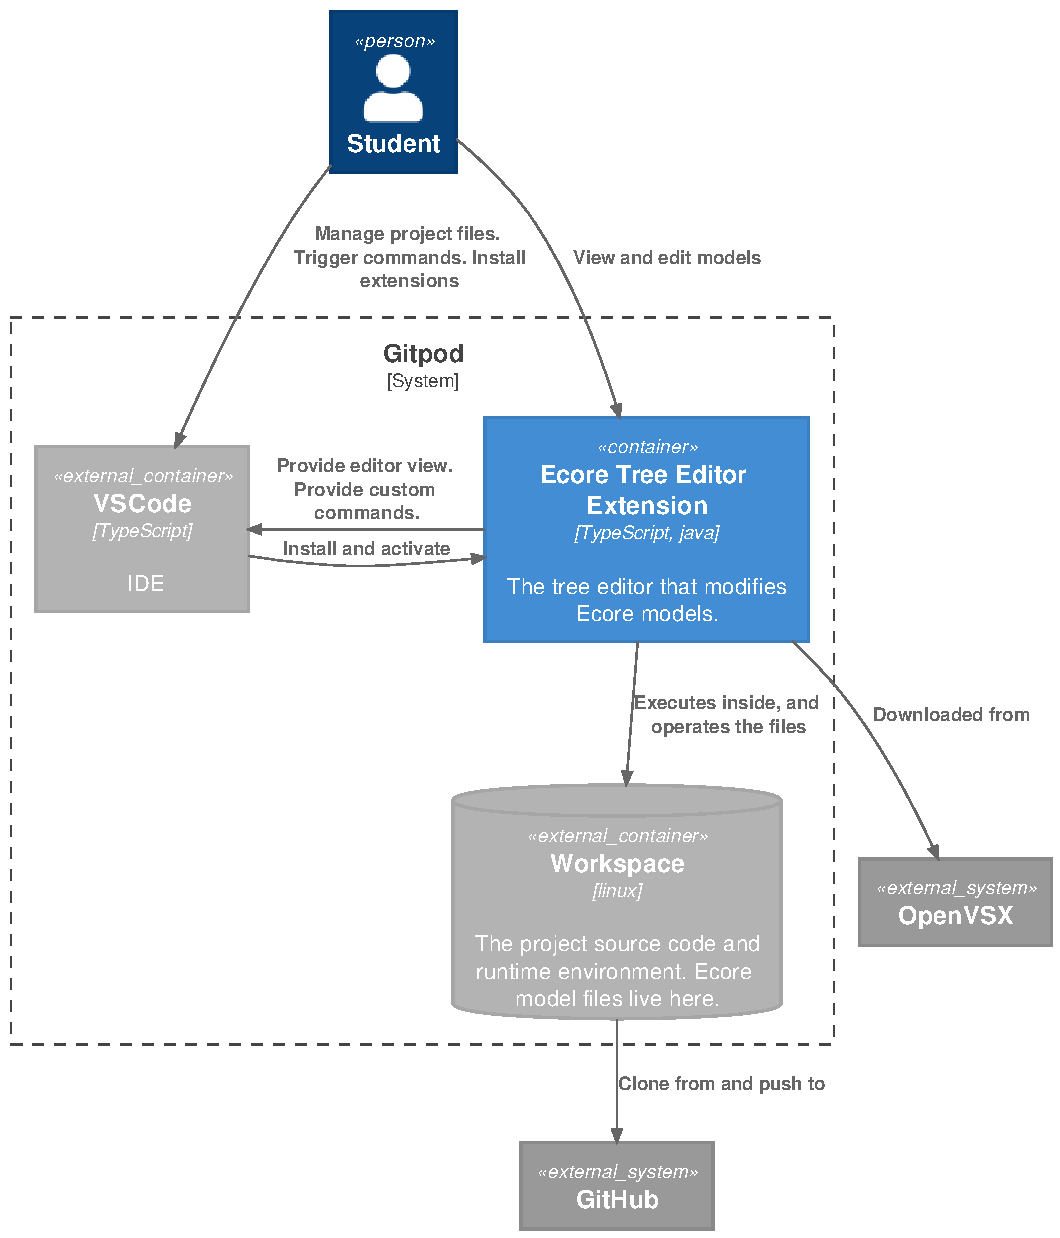
\includegraphics[width=\textwidth,height=\textheight,keepaspectratio]{figures/plantuml/Tree_Editor_Extension_container.pdf}
  \caption[Gitpod container diagram]{Container diagram for gitpod. The Gitpod system from \cref{fig:gitpod-system-context} is expanded to show its internal components. The \acrshort{IDE} used by Gitpod is \gls{Theia}.
  The student will interact with Theia, and install the Ecore Tree Editor Extension created from this thesis.
  This extension will also provide a user interface, which the student uses for modeling.
  This extension reads files from the Gitpod workspace, and uses the runtime provided by the workspace such as a Java Runtime Environment.}\label{fig:gitpod-container-diagram}
\end{figure}

\begin{figure}[htbp]  % order of priority: h here, t top, b bottom, p page
  \centering
  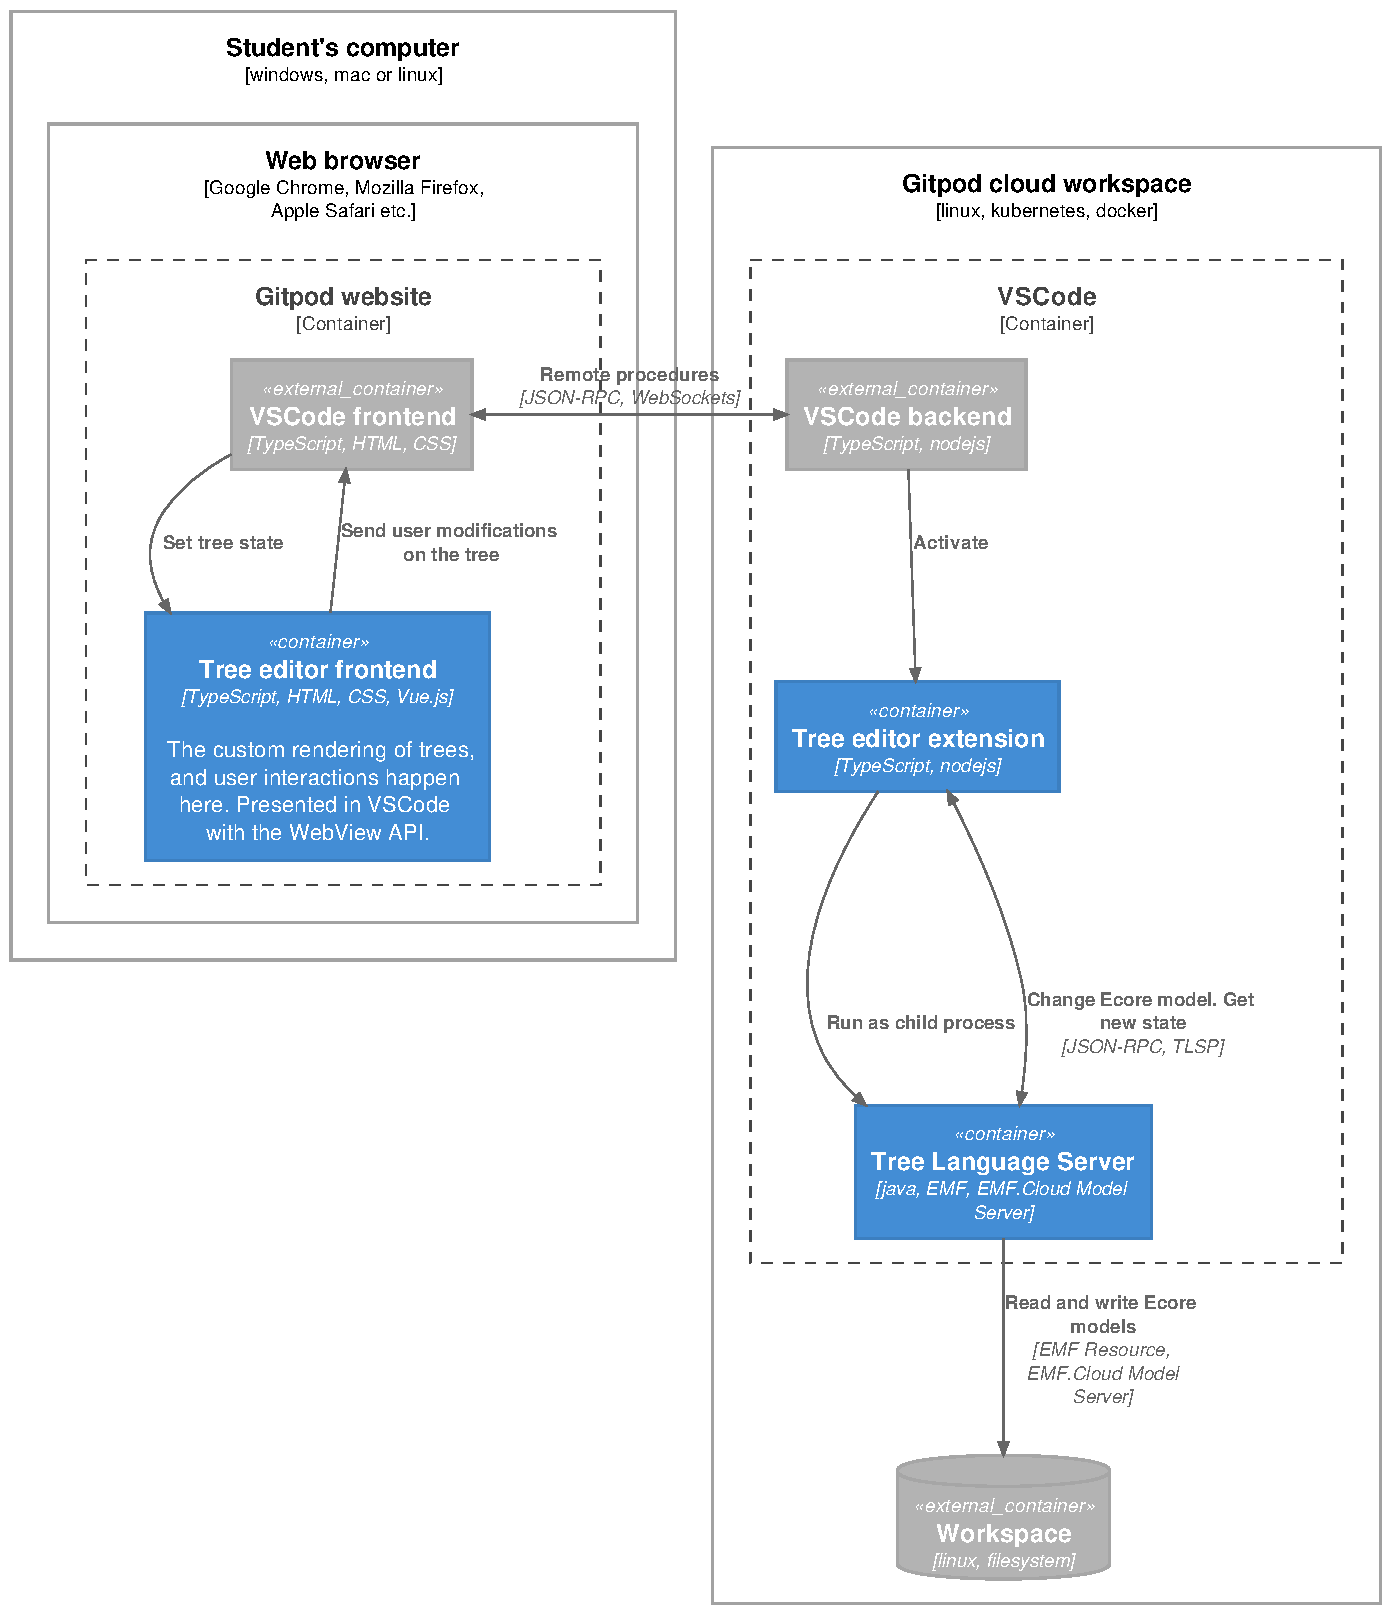
\includegraphics[width=\textwidth,height=\textheight,keepaspectratio]{figures/plantuml/Tree_Editor_Extension_deployment.pdf}
  \caption[Gitpod deployment diagram]{Deployment diagram of Gitpod. The student will use their computer to load the Gitpod website.
  The Gitpod service will start a computer in a cloud provider, to create a cloud workspace.
  The student only loads the Theia frontend and Tree editor frontend into their browser.
  Theia has a backend which runs inside the Workspace, and communicates to the frontend over WebSockets, using JSON-RPC\@.
  The Theia backend will activate the Tree editor extension, which in turn will start a Tree Language Server.
  This Tree Language Server runs java, and reuses the \acrshort{EMF} tooling.
  The Tree editor extension communicates to the Tree Language Server over a well defined protocol, where it asks to read model files, and execute commands to change the models.
  The Tree Language Server uses the Workspace to read and write \texttt{.ecore} files.}\label{fig:gitpod-deployment-diagram}
\end{figure}

\begin{figure}[htbp]  % order of priority: h here, t top, b bottom, p page
  \centering
  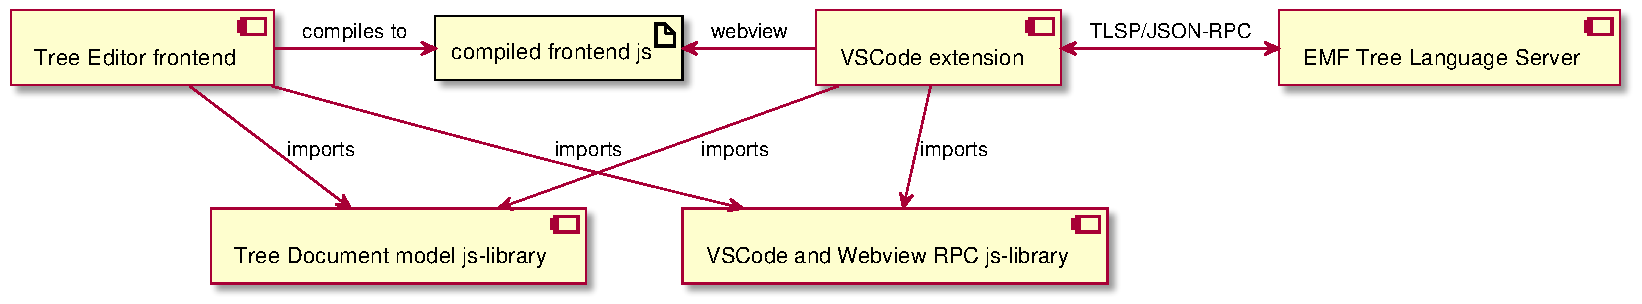
\includegraphics[width=\textwidth]{figures/plantuml/Tree_editor_components.pdf}
  \caption[Ecore Tree Editor component diagram]{Component diagram of the Ecore Tree Editor.
  The for the the extension is organized in 5 separate modules.
  The main module is the VSCode extension.
  This extension bundles the compiled frontend javascript artifact, and the compiled EMF Tree Language Server java jar-file.
  The Tree DOcument model js-library is the layer with the domain model for tree editors.
  It is used in both the frontend and the extension.
  }\label{fig:label4}
\end{figure}


\section{Design Artifact: Tree Language Server Protocol}\label{sec:tlsp}
% TODO



\newcommand{\bluearrowDesc}{The blue half-arrow ($\rightharpoondown$) is part of the \acrfull{TLSP}.}

\begin{figure}[htbp]  % order of priority: h here, t top, b bottom, p page
  \centering
  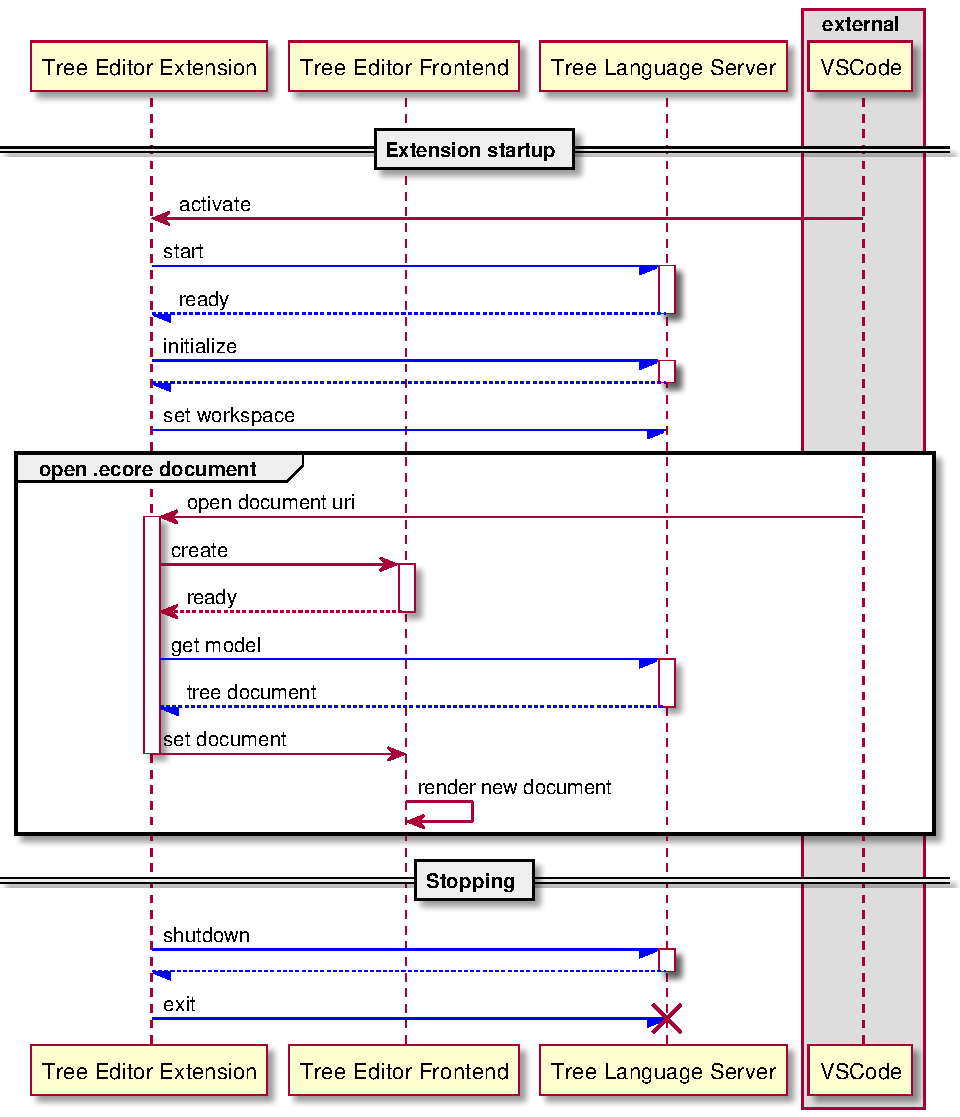
\includegraphics[width=\textwidth]{figures/plantuml/Protocol_startstop_sequence.pdf}
  \caption[Protocol Sequence Diagram of Start/Stop]{Sequence diagram for the protocol when starting and stopping the server. \bluearrowDesc}\label{fig:protocol-startstop}
\end{figure}

\begin{figure}[htbp]  % order of priority: h here, t top, b bottom, p page
  \centering
  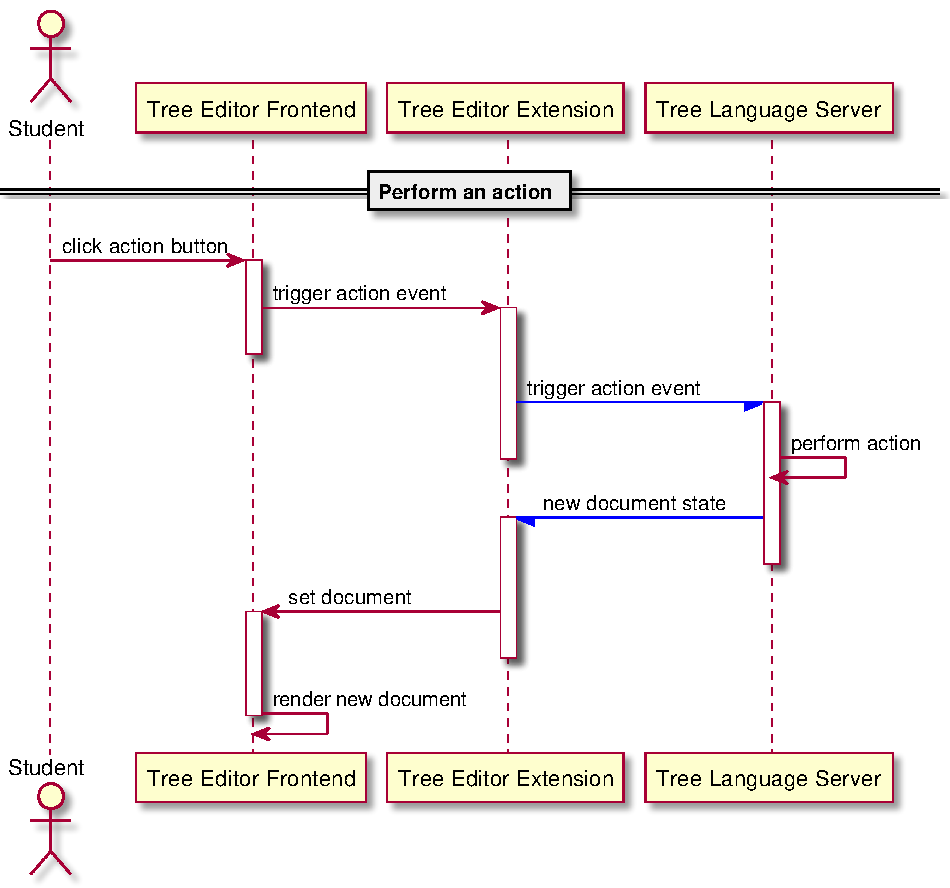
\includegraphics[width=\textwidth]{figures/plantuml/Protocol_action_sequence.pdf}
  \caption[Protocol Sequence Diagram of Action Triggering]{Sequence diagram for the protocol when triggering an action. \bluearrowDesc}\label{fig:protocol-action}
\end{figure}

\begin{figure}[htbp]  % order of priority: h here, t top, b bottom, p page
  \centering
  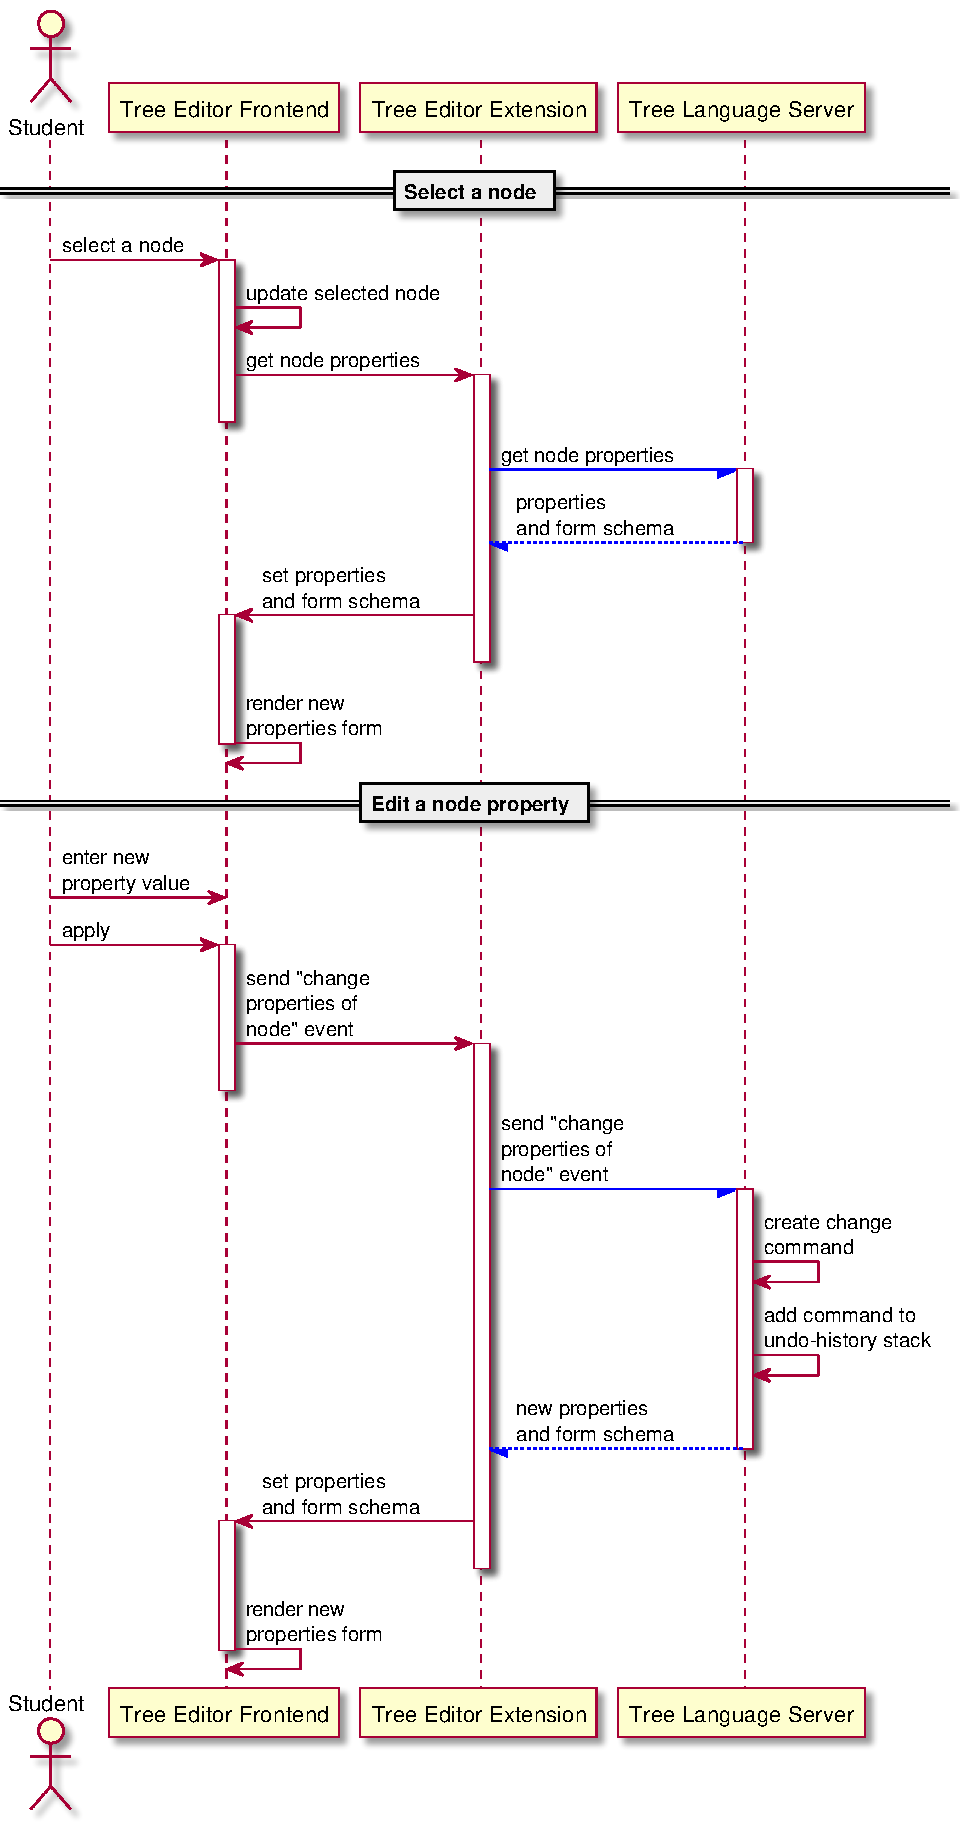
\includegraphics[width=\textwidth,height=\textheight,keepaspectratio]{figures/plantuml/Protocol_form_sequence.pdf}
  \caption[Protocol Sequence Diagram of Property Form]{Sequence diagram for the protocol when editing a node property. \bluearrowDesc}\label{fig:protocol-form}
\end{figure}

\begin{figure}[htbp]  % order of priority: h here, t top, b bottom, p page
  \centering
  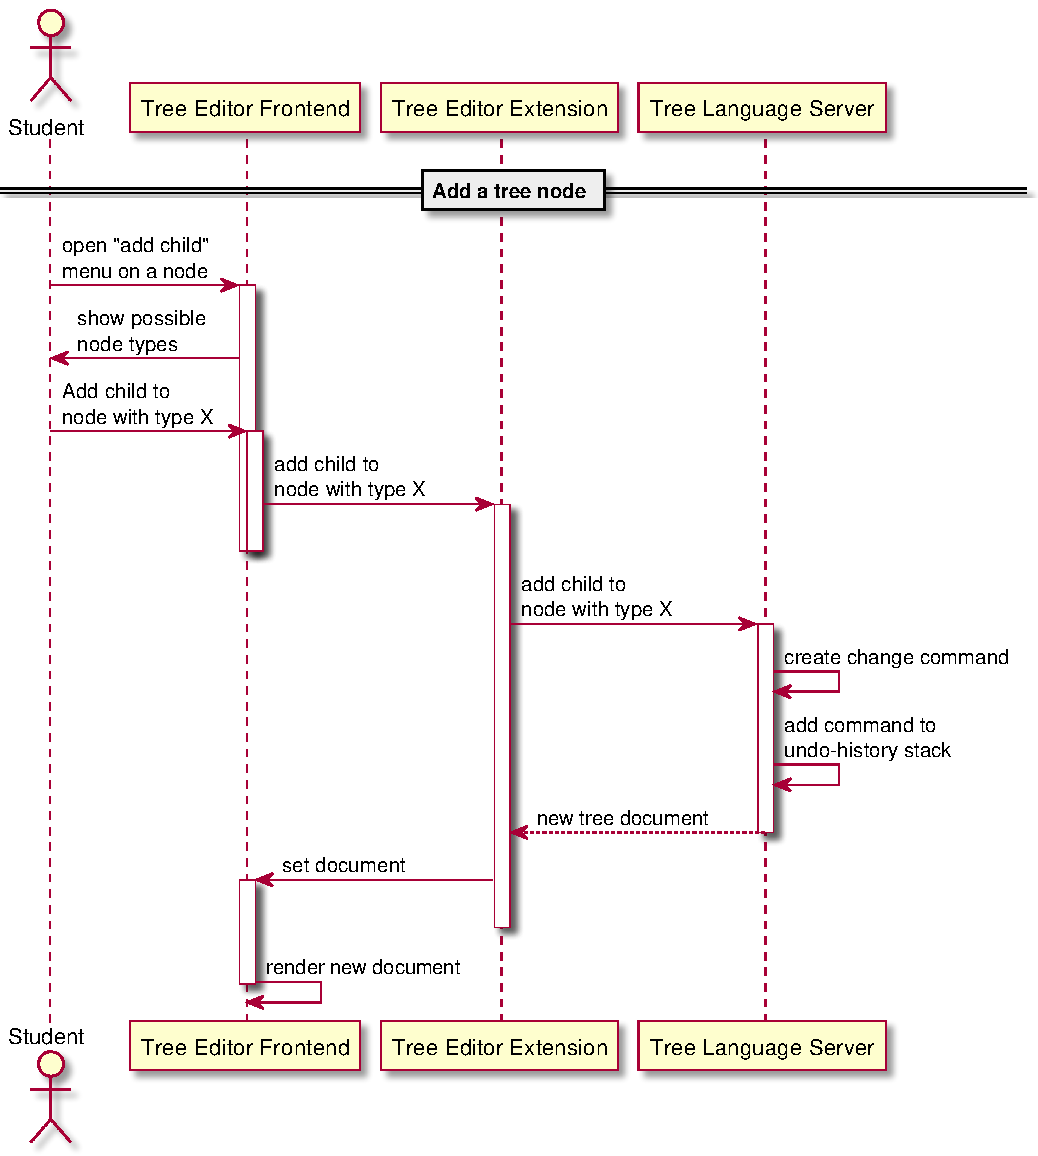
\includegraphics[width=\textwidth]{figures/plantuml/Protocol_changetree_sequence.pdf}
  \caption[Protocol Sequence Diagram of Tree Changes]{Sequence diagram for the protocol when adding a child node. \bluearrowDesc}\label{fig:protocol-changetree}
\end{figure}

\FloatBarrier



\section{Open Source Project: Measures Taken for Viability and Maintainability}


This section will describe the measures taken in order to make the project%
\footnote{The results report on the project in version \texttt{59b722c117}, available at \href{https://github.com/krissrex/tdt4900-master-thesis-ecore-tree-editor/tree/59b722c117346dcc53da16275819e0d5952f0d05}{\nolinkurl{https://github.com/krissrex/tdt4900-master-thesis-ecore-tree-editor/tree/59b722c117346dcc53da16275819e0d5952f0d05}}.}
viable and maintainable as an \gls{open source} project.

\subsection{Code Availability}

Possibly the most important part of \gls{open source}, is available source code.
The project is hosted%
\footnote{Project source: \href{https://github.com/krissrex/tdt4900-master-thesis-ecore-tree-editor}{\nolinkurl{https://github.com/krissrex/tdt4900-master-thesis-ecore-tree-editor}}.}
on a public website for collaboration on \gls{open source} software: \gls{GitHub}.

Also important, is the project visibility being \textit{public}, not private.

The project has the supervisor added as a contributor, in case one project maintainer is unavailable.

\subsection{Documentation}

\paragraph{Readme}
The main project has a ``Readme'' file with an overview of the project's components.

The components named ``tree-document-model-js'', ``tree-editor-frontend'', ``vscode-ecore-tree-editor-extension'' and ``vscode-webview-tree-editor-rpc'' have a Readme.
The ``model-server'' component does not have a Readme.\\

All the readme files are either very minimal, or the default Readme from a project generator.


\paragraph{Source code}
All the modules contain some comments inside the source code.
Not all the source code is documented, only where the author deemed it necessary.
A code base search%
\footnote{
\texttt{
ag --stats -c --ignore-dir dist '\textbackslash{}Q/**\textbackslash{}E\textbackslash{}s' .
}}
\lstinline{ag --stats -c --ignore-dir dist '\Q/**\E\s' .}
returned that 58 files of 169 files had comments, with a total of 128 comments.

\subsection{Automation}

\paragraph{Package manager}
A package manager is used for installing dependencies and compiling each module individually.
For the TypeScript modules, \texttt{npm} (Node Package Manager) is used, and dependencies are tracked in a \texttt{package.json}.
For the java module, \texttt{mvn} (Apache Maven) is used, and dependencies are tracked in a \texttt{pom.xml}.

\paragraph{Build}
Build scripts using \texttt{bash} are provided, that compile the modules (using npm or mvn) and copy the outputs to the correct path.
They also build in the correct order, regarding inter-module dependencies.

\paragraph{IDE configuration}
Files are added to automatically configure a contributor's \acrshort{IDE}, if they use \gls{VSCode} for the TypeScript modules and IntelliJ for the java module.
When using \gls{VSCode}, a list of recommended extensions is provided as well, which can be automatically installed.
There are \textit{Tasks} defined for \gls{VSCode} that can trigger the different npm builds, and \textit{Run configurations} to start the modules.

\paragraph{CI/CD}
There is no Continuous Integration (CI) and Continuous Deployment (CD) configured.
This can be added later when needed; for 1 developer it is overhead.

\subsection{Licensing}

\paragraph{Module license}
The modules use the MIT license\footnote{https://opensource.org/licenses/MIT}.
It is a very simple and permissive licence, compatible with \gls{open source}, and commonly used.
The licenses are not in separate files or the readme.
They are instead mentioned in the \texttt{package.json} and \texttt{pom.xml} files.

\paragraph{Copied code}
Some code is copied from other sources.
The original license has been included in these cases.
No code is copied from incompatible or strict licenses that contradict MIT.

\paragraph{Third party dependencies}
No proprietary dependencies are used%
\footnote{TypeScript modules were scanned with: \lstinline{npx license-checker --production}.}
, and none with incompatible or intrusive licenses.

\subsection{Code}

\paragraph{Code style}
The code uses readable names and small files.
The programming languages (TypeScript and Java) are common, especially in this context.
The code is formatted with automatic code formatters\footnote{Prettier and IntelliJ format the code.}, ensuring a consistent style.

\paragraph{Dependencies}
The dependencies and libraries used are common and in some cases official, in this context.
Effort has been put into using the same dependencies as related works (such as \acrshort{LSP} and EMF.Cloud projects).


\subsection{Issue Tracking}

An issue tracker is available on \gls{GitHub}.
A user is required, but signup is free.
A discussion forum is available as well on \gls{GitHub}.
There is no Wiki, but it is easy to create one on \gls{GitHub} if demand arises.


